\documentclass{article}

\usepackage{graphicx}

%% presentation style geometry to look like slides

\usepackage[%
  papersize={12.8cm,9.6cm},
  hmargin=1cm,%
  vmargin=1cm,%
  head=0.5cm,% might be changed later
  headsep=0pt,%
  foot=0.5cm% might be changed later
  ]{geometry}% http://ctan.org/pkg/geometry

\begin{document}
\newpage
   \vspace*{\stretch{1.0}}
   \begin{center}
      \Large\textbf{Earth 436B Thesis}\\
      \large\textit{John Lawson}
   \end{center}
   \vspace*{\stretch{2.0}}

\newpage



\section{Introduction}
-Movement of Earths crust atop the mantle is driven by many factors including buoyancy\\
-Addition and removal of weight, in this case the Laurentide Ice Sheet, from the crust will cause vertical adjustments known as GIA\\
-As inclination of ground surface changes, water levels (ie Lakes) and the paths taken by
the flow of water (rivers, lake outlets, groundwater) change\\
-This has implications for engineering and environmental assessments\\
-projection of future changes due to GIA relies on having a reliable estimate of
past rates of GIA\\
% cant infer long term process from short term data
% mention past efforts using water gauges, gps data
\newpage

\section[2]{Previous Work}
-OSL dating used to determine age for sequences of Quaternary beach deposits (strandplain sequences) at each site vs current day elevation.\\
-This is then used to create a graph of elevation vs time for each site\\
-Paleohydrographs were created in Johnston et al. 2012
\newpage
\section{Locations}   
-Grand Traverse Bay, Michigan (GTB)\\
-Au Train Bay, Michigan (ATB)\\
-Batchawana Bay, Ontario (BATB)\\
-Tahquamenon Bay, Michigan (TAHB)\\
\\
\begin{figure}[h]
	\makebox[\textwidth]{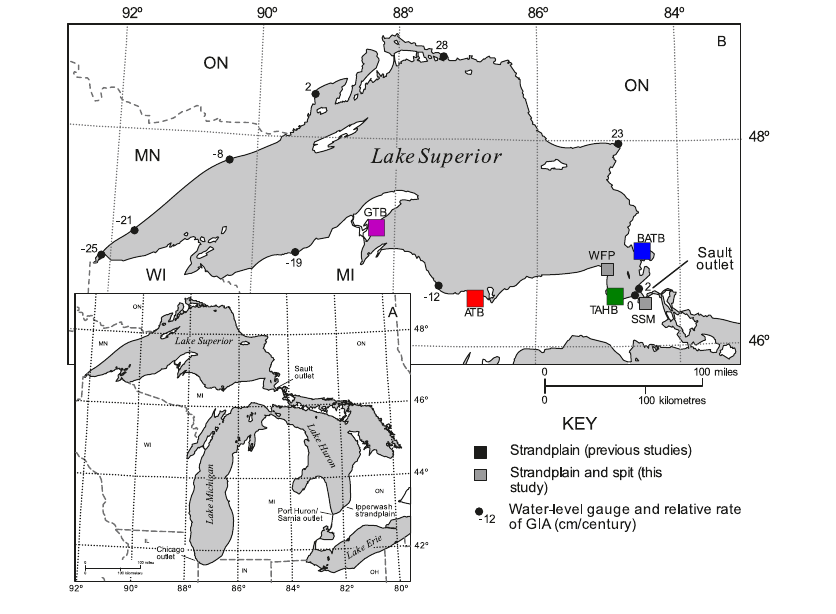
\includegraphics[width=0.72\paperwidth]{johnstonLaurentianMap.png}}
	\caption{Map of the study sites used. Reproduced with permission from Johnston et al. 2012}
	\label{fig:jj2012map}
\end{figure}

\newpage


% add map, maybe with data points
\newpage
% talk about location
% talk about link between importance of water levels and they cant be understood
% without understanding gia
% talk about what gia is
\begin{figure}[h]
	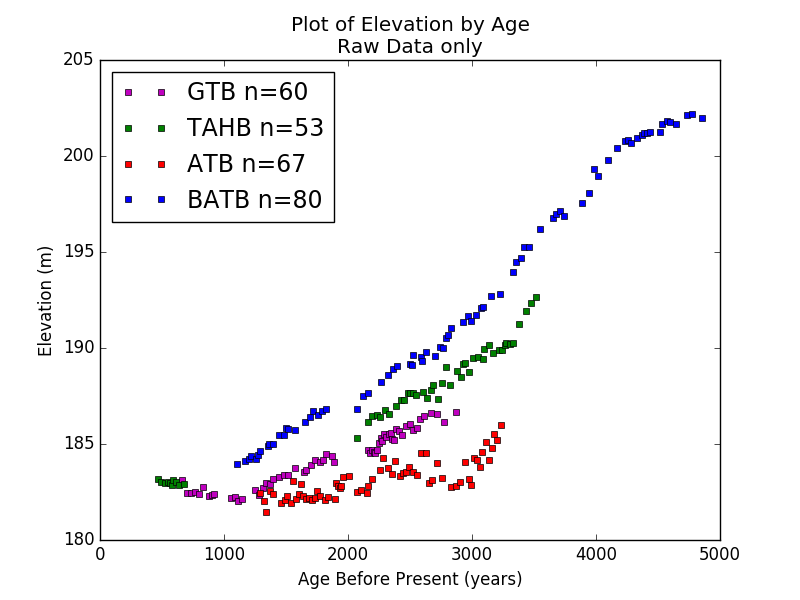
\includegraphics[width=1.1\linewidth]{data/theDataRaw.png}
	\caption{Current day elevation of relict shorelines with respect to time before present over the last 5000 years. Strandplain sites Au Train Bay, Michigan (ATB), Batchawana Bay, Ontario (BATB), Tahquamenon Bay, Michigan (TAHB), and Grand Traverse Bay, Michigan (GTB) surrounding Lake Superior are plotted individually. Data from Johnston et al, (2012)}
	\label{fig:rawData}
\end{figure} 
%\begin{figure}[h]
	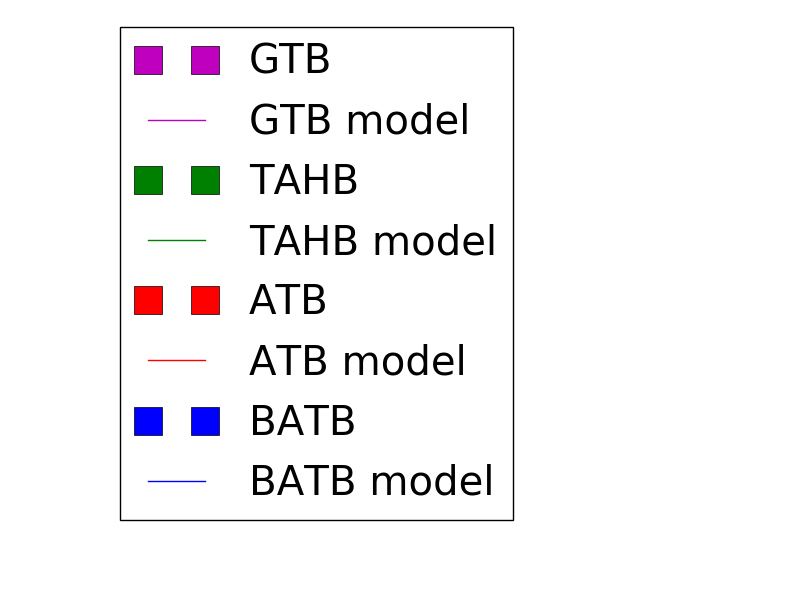
\includegraphics[width=0.40\textwidth]{data/legendary.png}
	%\makebox[\textwidth]{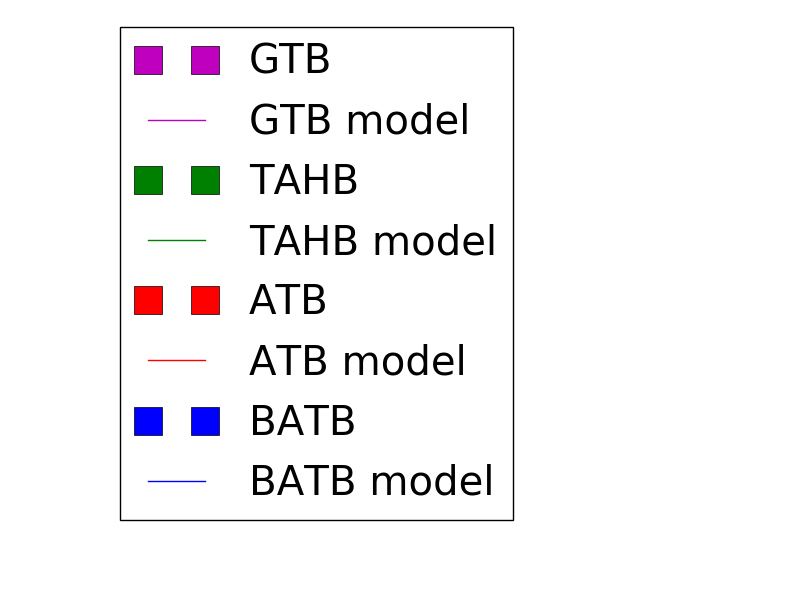
\includegraphics[width=\paperwidth]{data/legendary.png}}
	%\caption{Site Legend}
	%\label{fig:rdmLegend}
\end{figure}


% talk about structure of data, what are axes, why is it increasing
% talk about objective
\newpage
\section[2]{Method}
-Johnston et al. 2012 used a linear regression method for each site to get relative GIA rates between sites\\
-Model is likely too simplistic and doesnt take account of local variations\\
-Data not available continuously for each site, or at the same time for each site to compare gia, so values must be inferred using linear interpolation between known data points.\\
\begin{figure}[h]
	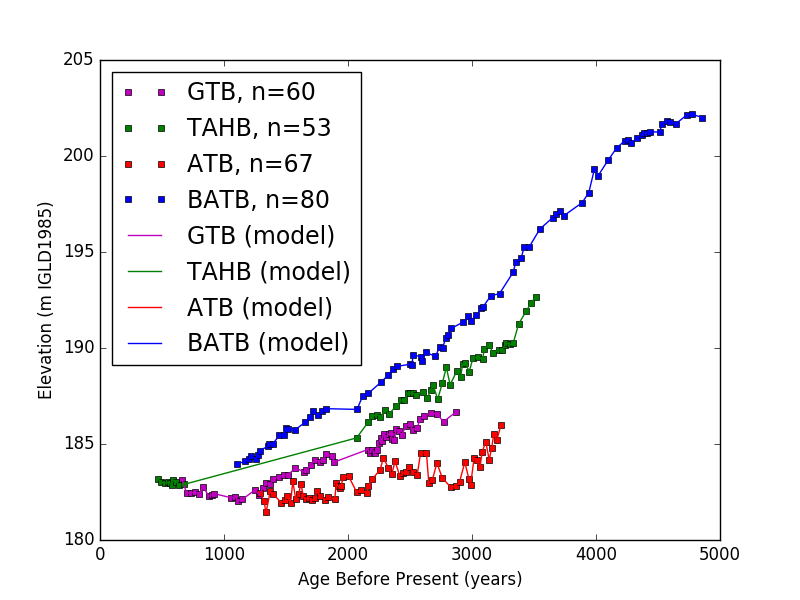
\includegraphics[width=\linewidth]{data/theData.png}
	\caption{Water surface elevation with respect to time before present, modelled}
	\label{fig:rawDataWithModel}
\end{figure}
\newpage
%\begin{figure}[h]
	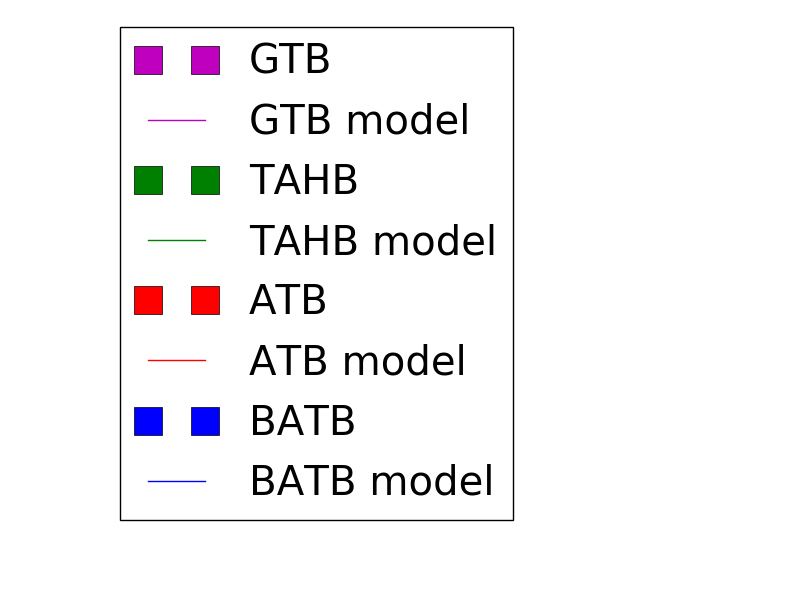
\includegraphics[width=0.40\textwidth]{data/legendary.png}
	%\makebox[\textwidth]{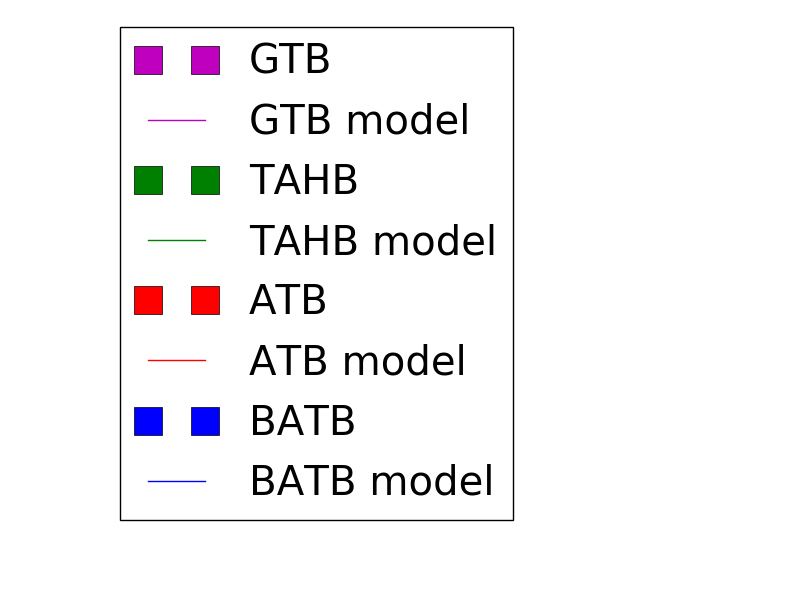
\includegraphics[width=\paperwidth]{data/legendary.png}}
	%\caption{Site Legend}
	%\label{fig:rdmLegend}
\end{figure}


% note mainville & craymer, previous work has used water level gauge data, but
% cant infer a long term process from short term data
\newpage
\section[2]{Method}
-GIA is now plotted by subtracting between the measured values of one dataset and the modelled value of another.\\
-6 combinations of pairs of sites are created, each of which has a forward (A to B) and backward (B to A) comparison.\\
\newpage
%\section{Previous Work} 
Mainville \& Craymer (2005) used water gauge data collected around the LGL over the past 150 years to
 create monthly means of water level. Differences in these values between sites
 were then plotted against time to calculate a rate of elevation change between
 sites over time (This value is interpreted to represent the impact of the GIA
 process on the crust underlying the LGL, even though the actual process extends
 over a much longer timescale than that of the data collection). Combinations of sites were shown to produce
 inconsistent results, so a second method using a least squares adjustment process was used,
 removing some monthly mean outliers which plotted at or beyond some arbitrary residual distance away 
 from the linear regression line in the vertical (elevation) axis. 
 This process was repeated with each new linear regression on the remaining data
 points until none remained "too far away" from
 the final regression line. A third, and ultimately optimal method for calculating
 GIA was developed by
 Mainville \& Craymer in their 2005 paper, this time computing velocity at a given
 month from the difference between a
 the monthly water level mean and an reference water level for the epoch that the 
 month is found in (this 
 reference level being adjusted for epoch
 and site biases). This elevation difference is then divided by the time difference
 between the start of the epoch and the month that was measured, calculating a rate
 of GIA for the month measured. Their findings with this method showed a general agreement with the post glacial
 ICE-3G global model of GIA at that time, while the ICE-4G model developed by Peltier
 was shown to underestimate the relative difference in vertical movement across
 the span of the Great Lakes (Mainville \& Craymer, 2005).\\ \\
Johnston et al. (2012) attempted to provide a value for GIA in the LGL with
 better accuracy than previous estimates calculated using water
 gauge data.
 
In order to accomplish this, the data used to measure the process of
 GIA needed to extend over a much longer timescale. In this method, water
 levels were inferred from the elevation of relict shorelines in beach ridge
 strandplains from the late Holocene sediment record surrounding Lake Superior.
 Ages for each elevation were inferred from age dating samples from these beach
 deposits (known as strandplain sequences) using
 optically stimulated luminescence (OSL) age dating. Johnston et al (2012) differed from
 Mainville \& Craymer (2005), in that data collected for the 2012 paper using OSL
 age dating did not have
 elevations sampled at the same points in time for calculation of relative
 rates. As a result, Johnston et al (2012) the elevation vs time data was modelled with a linear
 regression for each site, the difference in slopes of each regression representing the GIA rate
 between sites. Individual regressions were further created per site
 for a series of four ranges of time related to lake level phases, namely the Nipissing,
 Algoma, Sault, and Sub-Sault (Johnston et al, 2012). The results reported from this process
 are summarized in Figure \ref{fig:jj2012Grid}. \\
 
 \begin{figure}[t]
	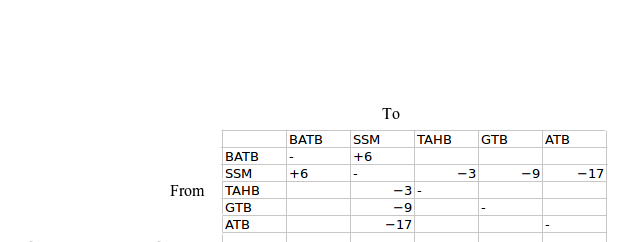
\includegraphics[width=0.9\linewidth]{jjGrid.png}
	\caption{GIA values reported by Johnston et al 2012. All values are in cm/century.}
	\label{fig:jj2012Grid}
 \end{figure}
 % need to ask JJ about JJ 2012, bottom of page 3, divergence of intercepts
 



\newpage
\begin{figure}[t]
	\makebox[\textwidth]{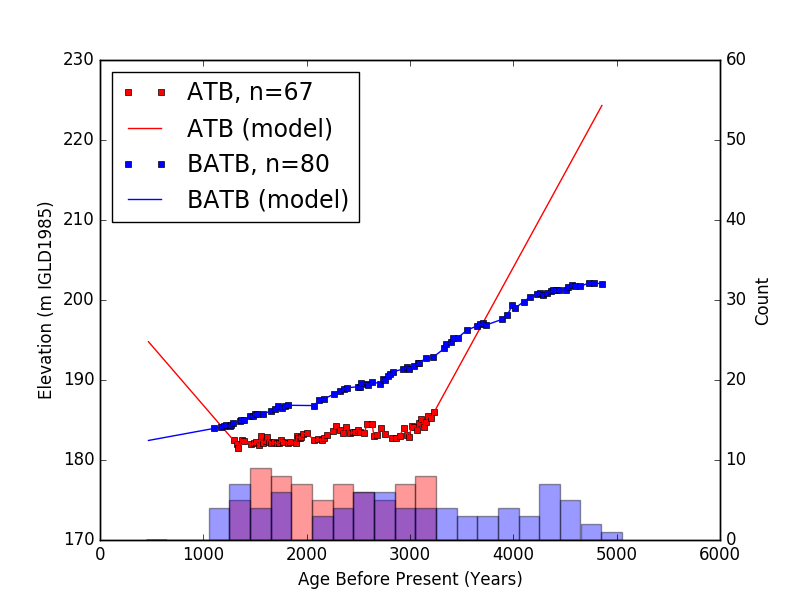
\includegraphics[width=0.72\paperwidth]{data/ATB-BATB_DataAndModel.png}}
	\caption{ATB-BATB raw data with linear interpolation model}
	\label{fig:data_ATBxBATB}
\end{figure}
\newpage

\begin{figure}[t]
	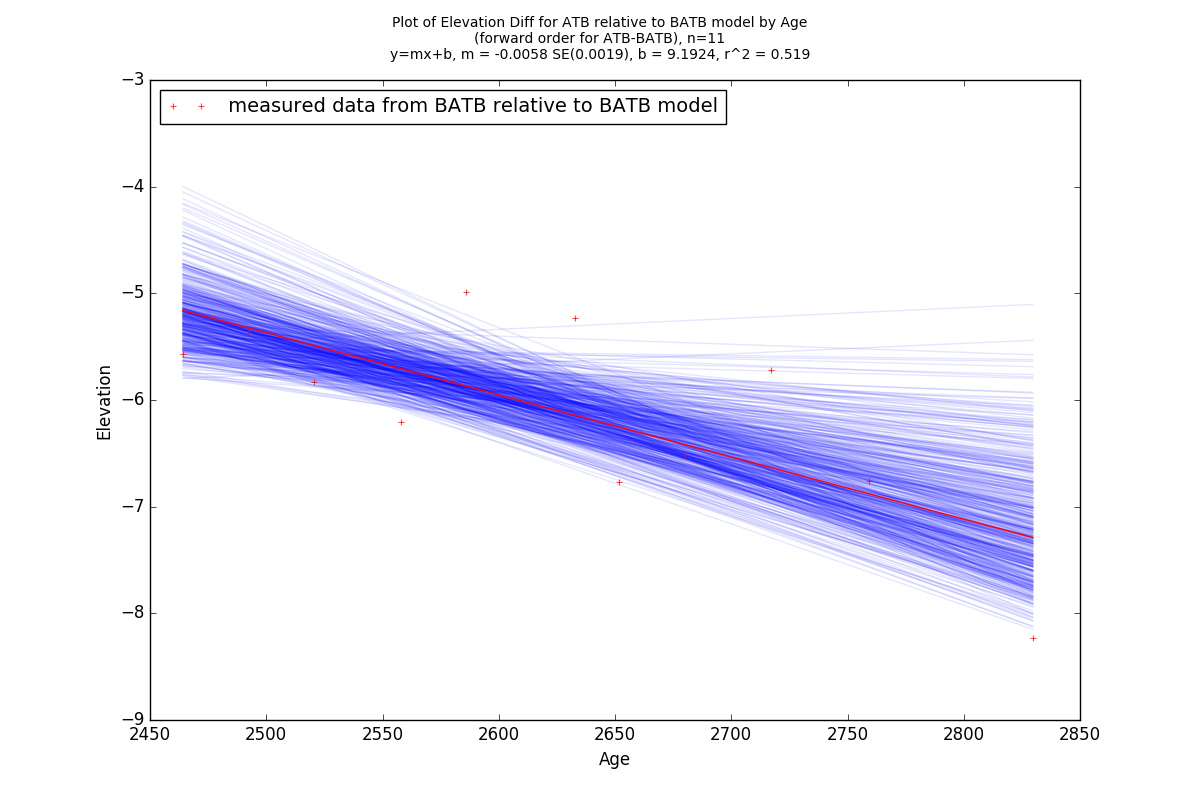
\includegraphics[width=0.9\linewidth]{data/gias/theGIA_ATB_relative_to_BATB.png}
	\caption{Differences in elevation measured from the ATB data to the ATB model}
	\label{fig:gias_ATBxBATB}
\end{figure}
\newpage


\begin{figure}[t]
	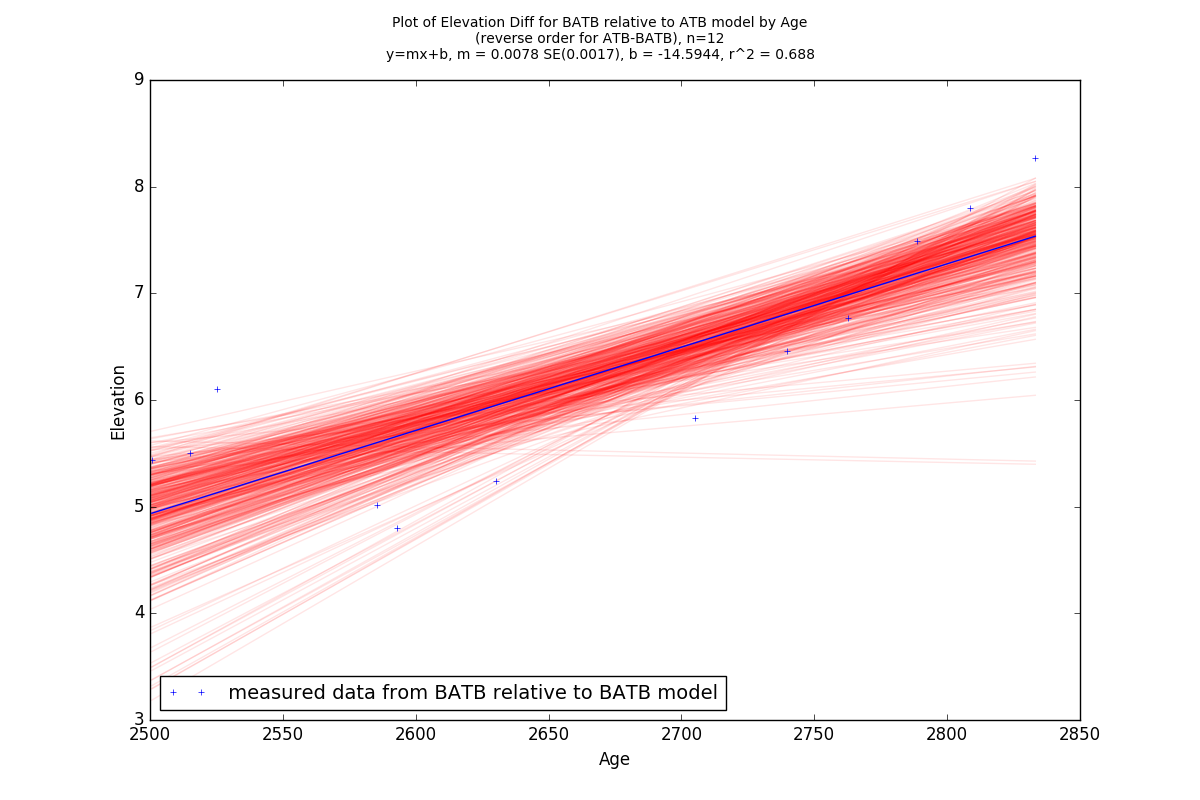
\includegraphics[width=0.9\linewidth]{data/gias/theGIA_BATB_relative_to_ATB.png}
	\caption{Differences in elevation measured from the BATB data to the ATB model}
	\label{fig:gias_BATBxATB}
\end{figure}
\newpage
% this desperately needs to be done as a loop



\begin{figure}[h]
	\makebox[\textwidth]{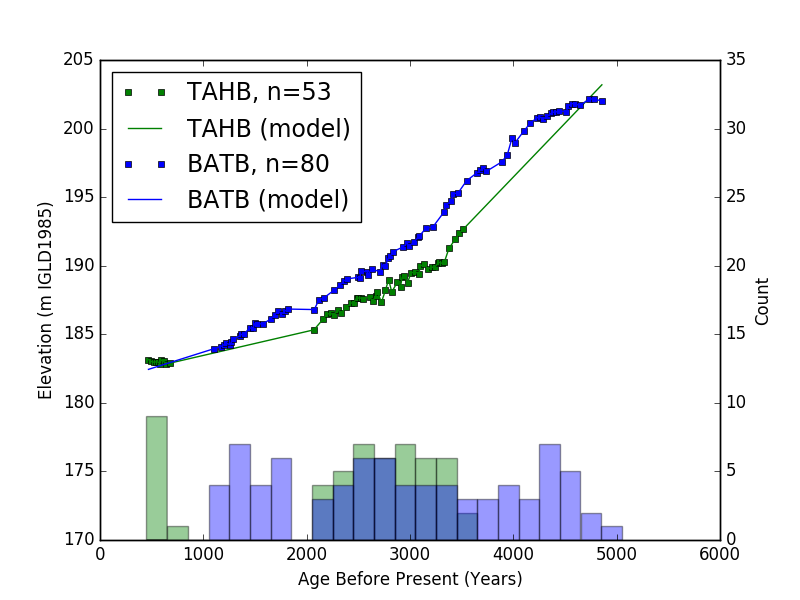
\includegraphics[width=0.72\paperwidth]{data/TAHB-BATB_DataAndModel.png}}
	\caption{TAHB-BATB raw data with linear interpolation model}
	\label{fig:data_TAHBxBATB}
\end{figure}
\newpage

\begin{figure}[h]
	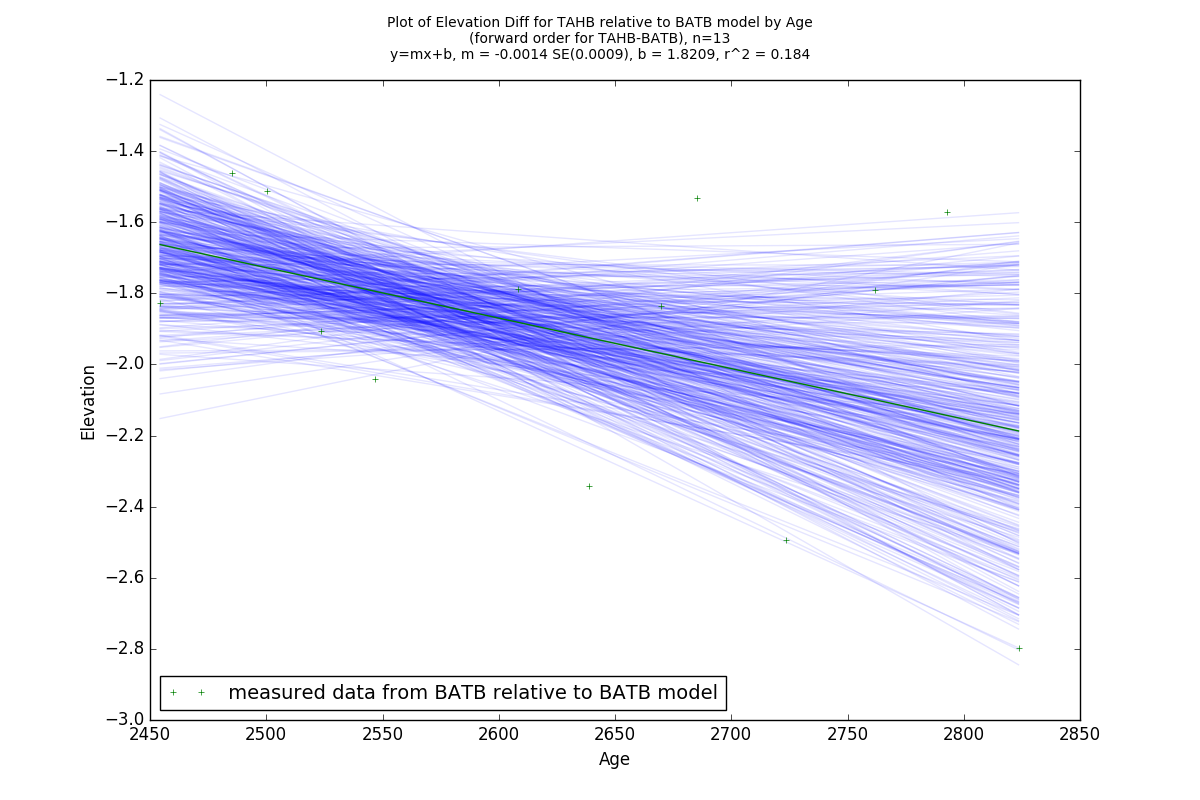
\includegraphics[width=0.9\linewidth]{data/gias/theGIA_TAHB_relative_to_BATB.png}
	\caption{Differences in elevation measured from the TAHB data to the BATB model}
	\label{fig:gias_TAHBxBATB}
\end{figure}
\newpage


\begin{figure}[h]
	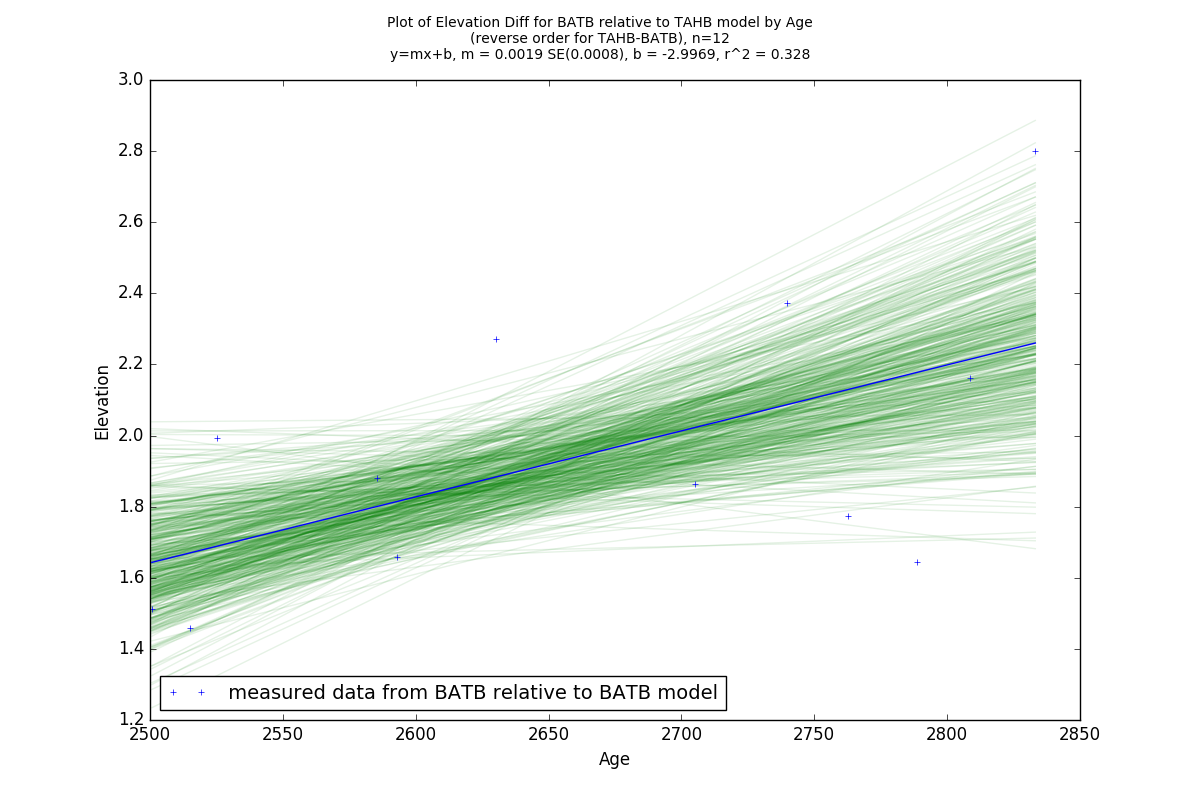
\includegraphics[width=0.9\linewidth]{data/gias/theGIA_BATB_relative_to_TAHB.png}
	\caption{Differences in elevation measured from the BATB data to the TAHB model}
	\label{fig:gias_BATBxTAHB}
\end{figure}
\newpage








\begin{figure}[h]
	\makebox[\textwidth]{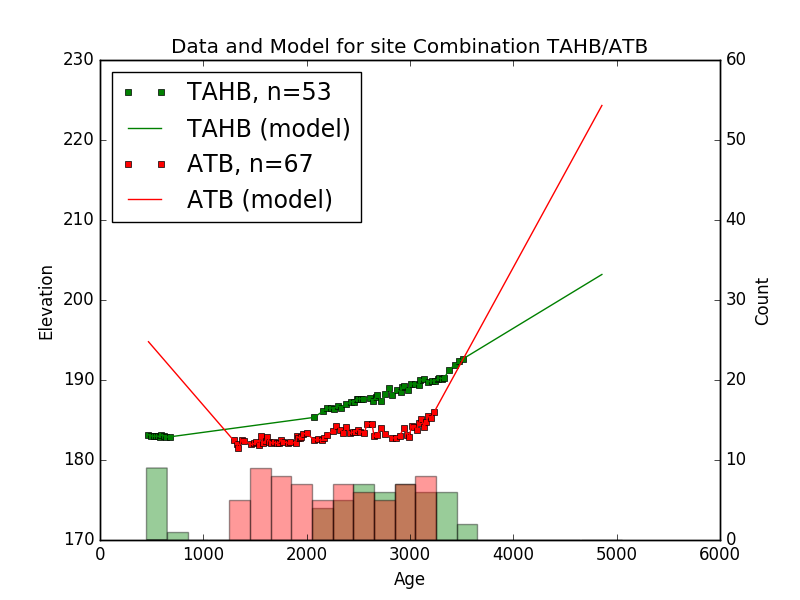
\includegraphics[width=0.72\paperwidth]{data/TAHB-ATB_DataAndModel.png}}
	\caption{TAHB-ATB raw data with linear interpolation model}
	\label{fig:data_TAHBxATB}
\end{figure}
\newpage

\begin{figure}[h]
	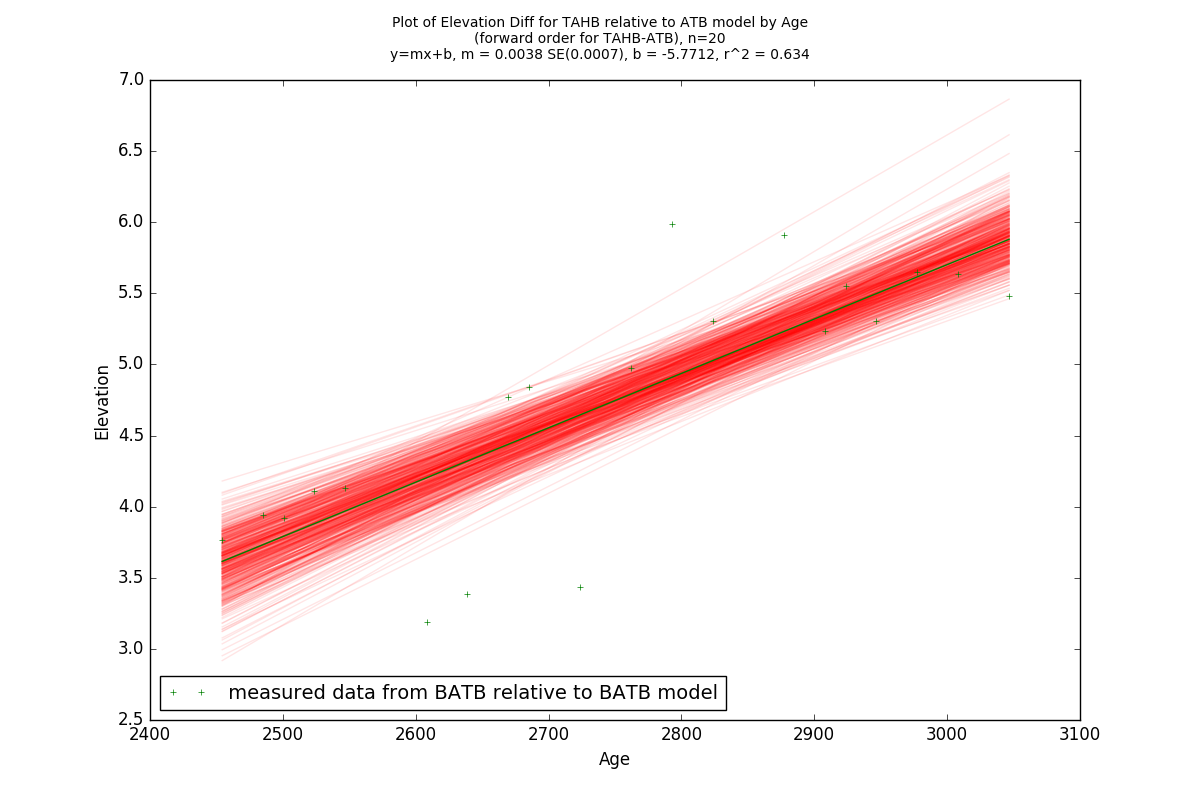
\includegraphics[width=0.9\linewidth]{data/gias/theGIA_TAHB_relative_to_ATB.png}
	\caption{Differences in elevation measured from the TAHB data to the ATB model}
	\label{fig:gias_TAHBxATB}
\end{figure}
\newpage


\begin{figure}[h]
	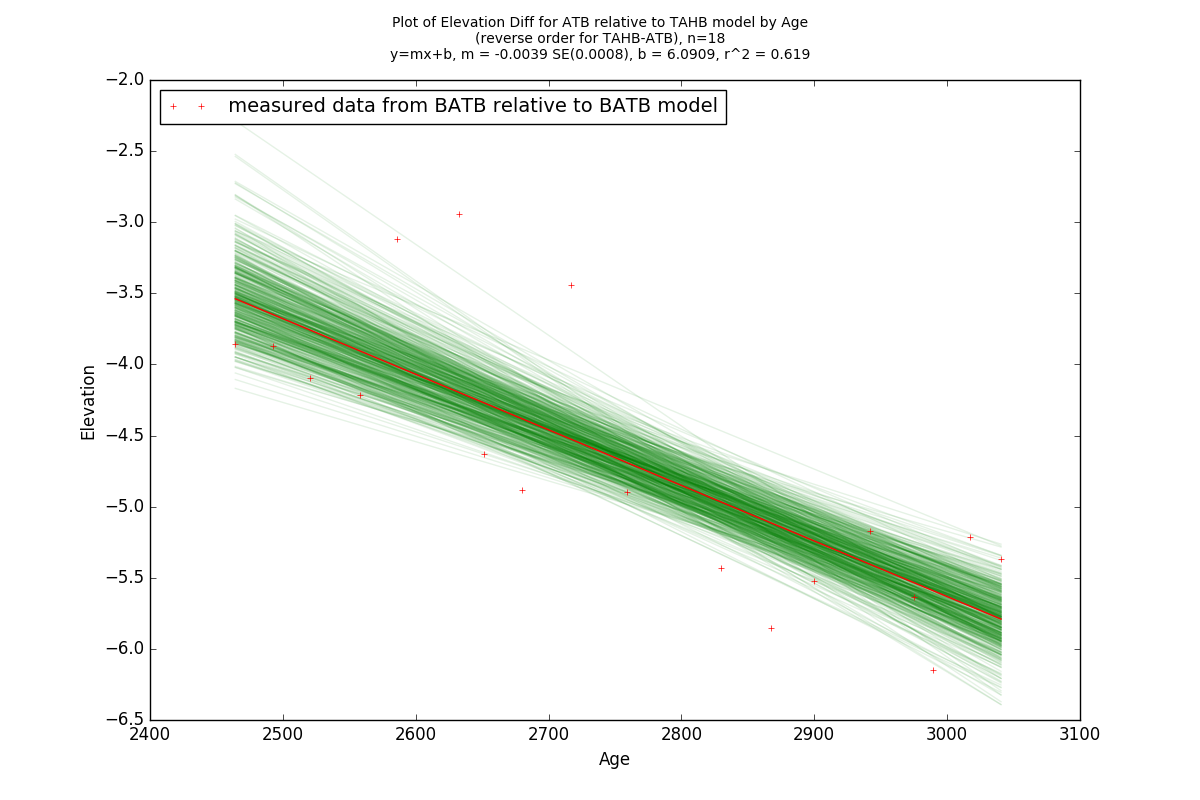
\includegraphics[width=0.9\linewidth]{data/gias/theGIA_ATB_relative_to_TAHB.png}
	\caption{Differences in elevation measured from the ATB data to the TAHB model}
	\label{fig:gias_ATBxTAHB}
\end{figure}
\newpage






\begin{figure}[h]
	\makebox[\textwidth]{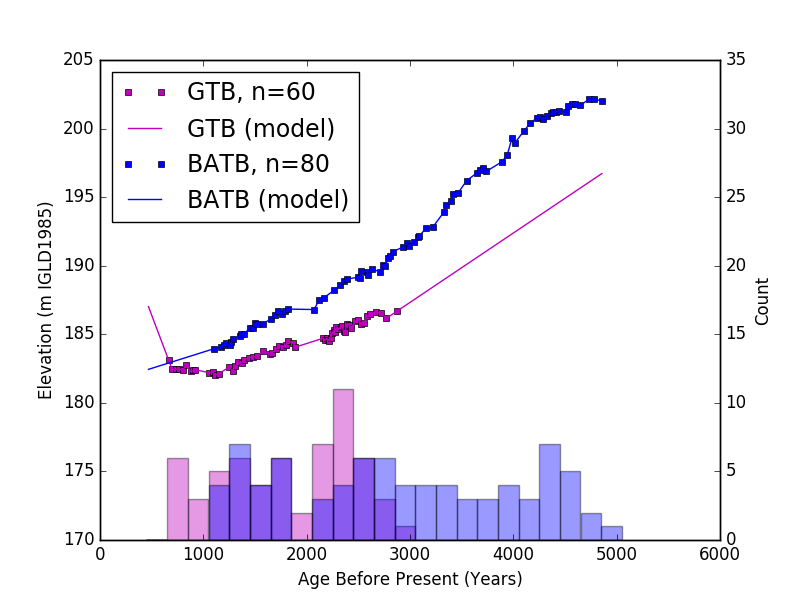
\includegraphics[width=0.72\paperwidth]{data/GTB-BATB_DataAndModel.png}}
	\caption{GTB-BATB raw data with linear interpolation model}
	\label{fig:data_GTBxBATB}
\end{figure}
\newpage

\begin{figure}[h]
	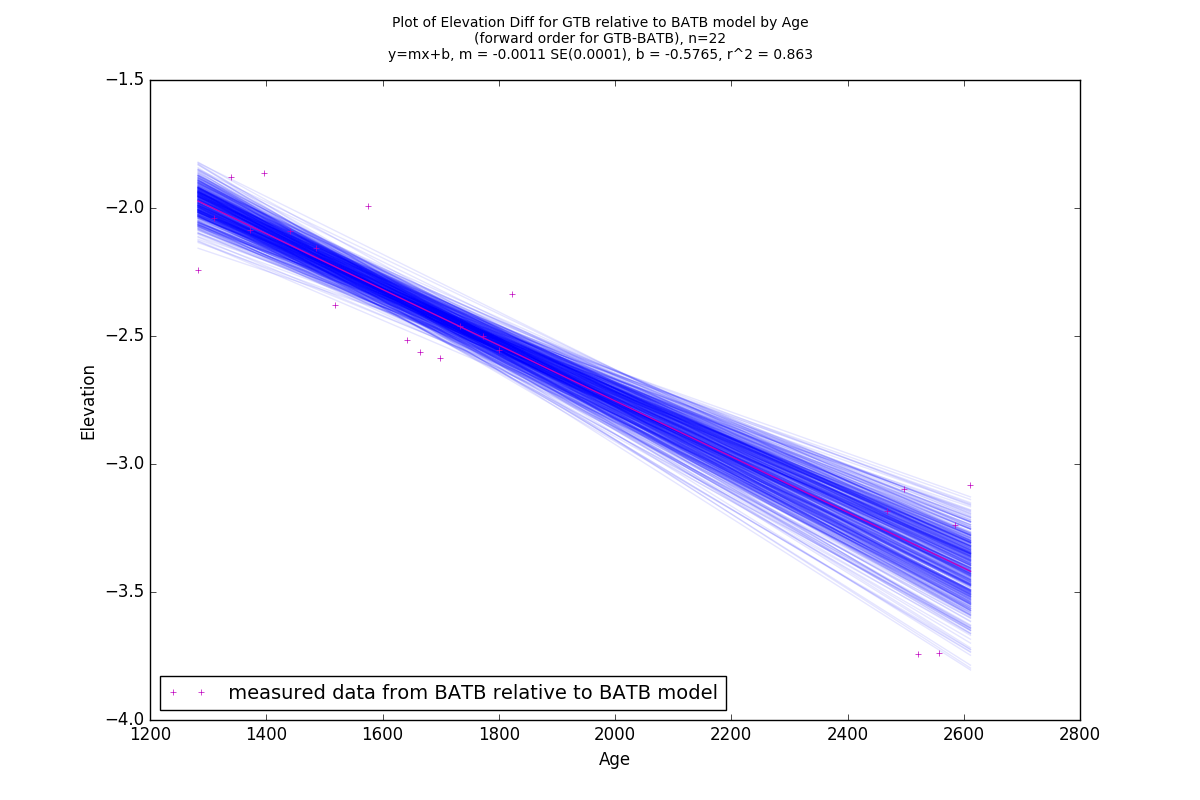
\includegraphics[width=0.9\linewidth]{data/gias/theGIA_GTB_relative_to_BATB.png}
	\caption{Differences in elevation measured from the GTB data to the BATB model}
	\label{fig:gias_GTBxBATB}
\end{figure}
\newpage


\begin{figure}[h]
	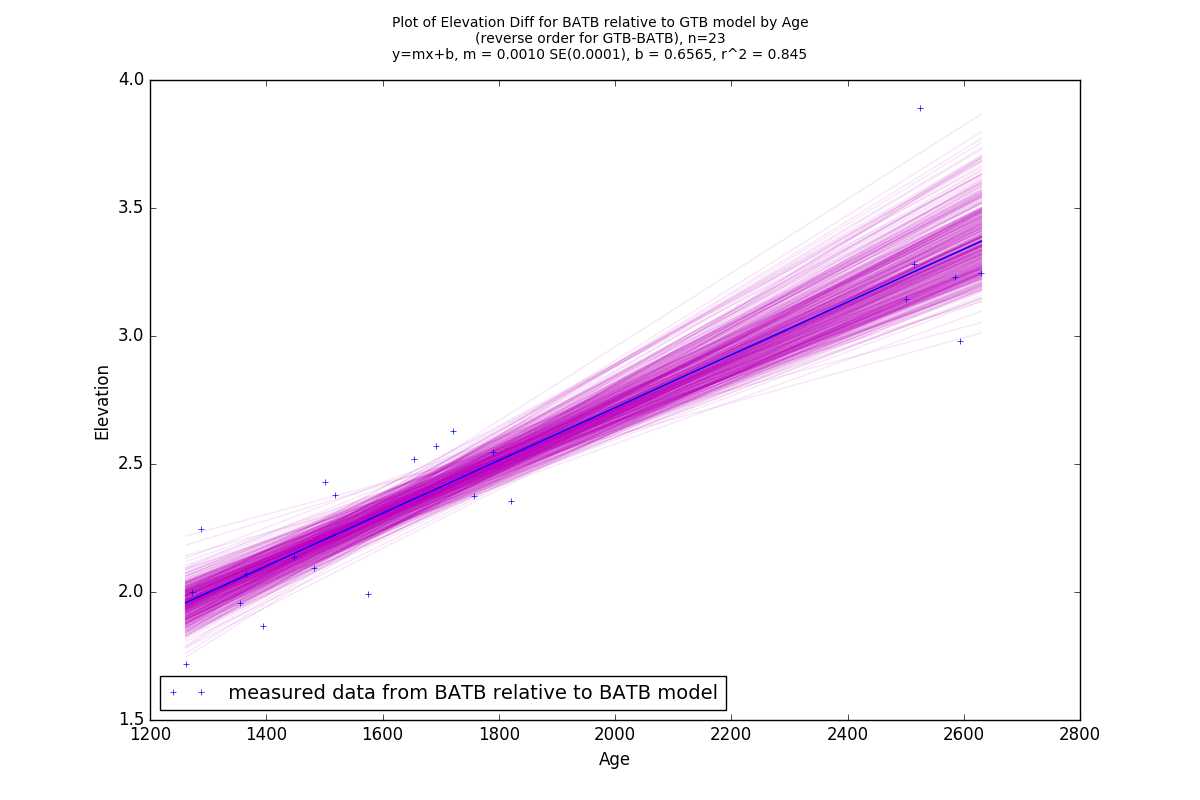
\includegraphics[width=0.9\linewidth]{data/gias/theGIA_BATB_relative_to_GTB.png}
	\caption{Differences in elevation measured from the BATB data to the GTB model}
	\label{fig:gias_BATBxGTB}
\end{figure}
\newpage









\begin{figure}[h]
	\makebox[\textwidth]{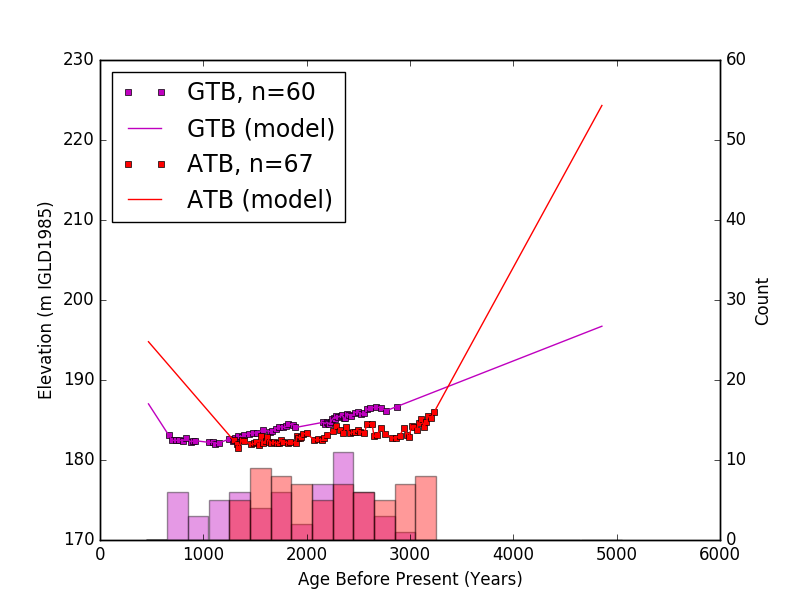
\includegraphics[width=0.72\paperwidth]{data/GTB-ATB_DataAndModel.png}}
	\caption{GTB-ATB raw data with linear interpolation model}
	\label{fig:data_GTBxATB}
\end{figure}
\newpage

\begin{figure}[h]
	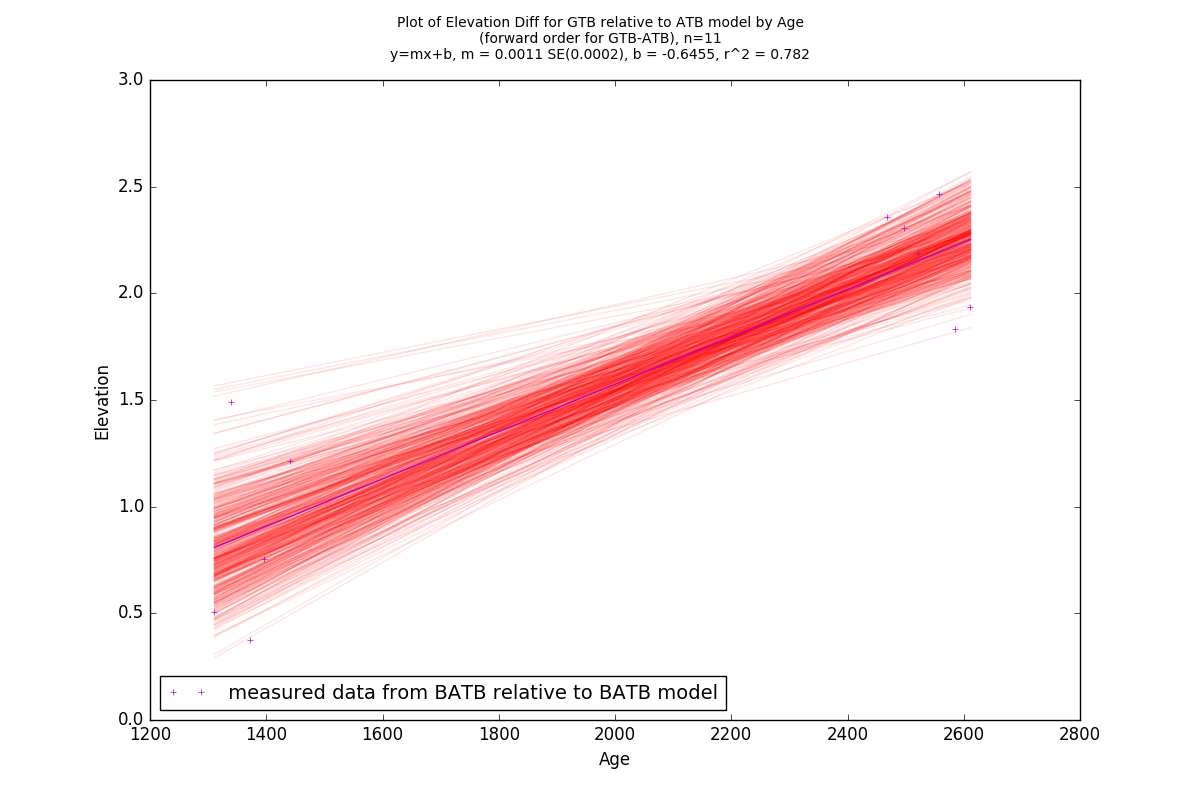
\includegraphics[width=0.9\linewidth]{data/gias/theGIA_GTB_relative_to_ATB.png}
	\caption{Differences in elevation measured from the GTB data to the ATB model}
	\label{fig:gias_GTBxATB}
\end{figure}
\newpage


\begin{figure}[h]
	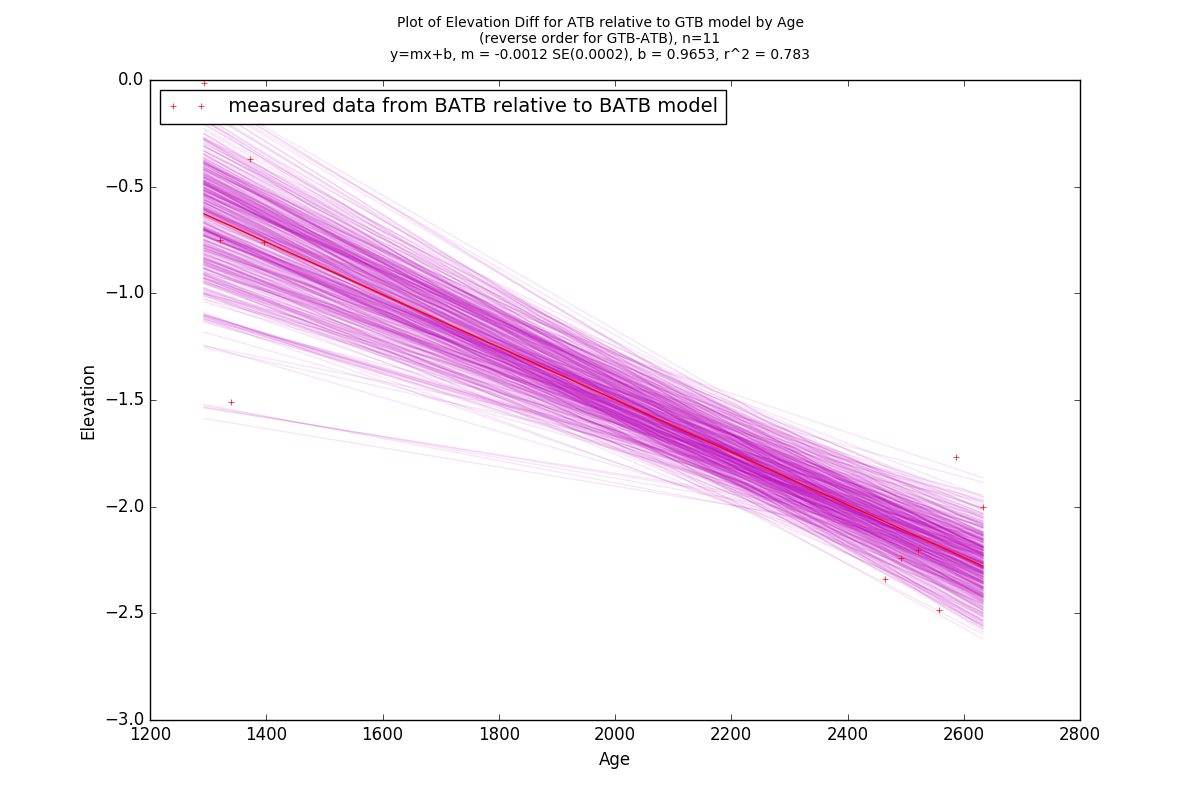
\includegraphics[width=0.9\linewidth]{data/gias/theGIA_ATB_relative_to_GTB.png}
	\caption{Differences in elevation measured from the ATB data to the GTB model}
	\label{fig:gias_ATBxGTB}
\end{figure}
\newpage










\begin{figure}[h]
	\makebox[\textwidth]{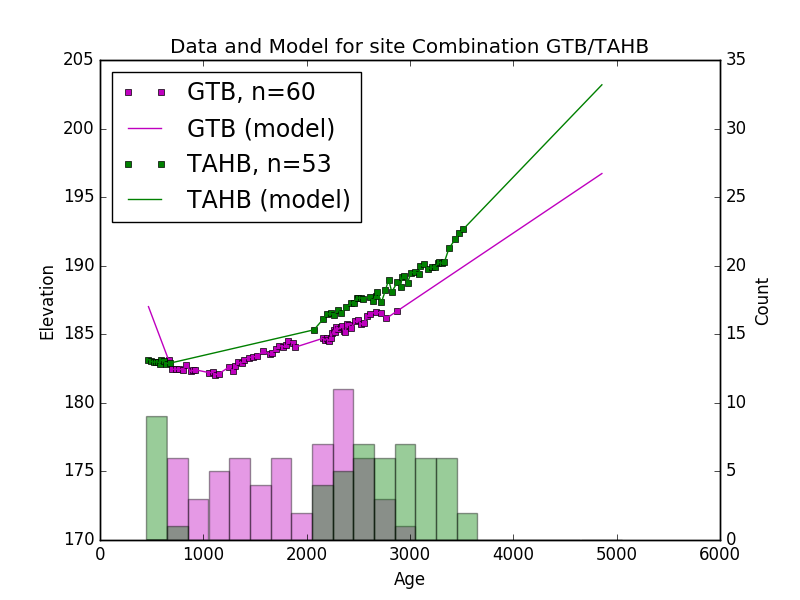
\includegraphics[width=0.72\paperwidth]{data/GTB-TAHB_DataAndModel.png}}
	\caption{GTB-TAHB raw data with linear interpolation model}
	\label{fig:data_GTBxTAHB}
\end{figure}
\newpage

\begin{figure}[h]
	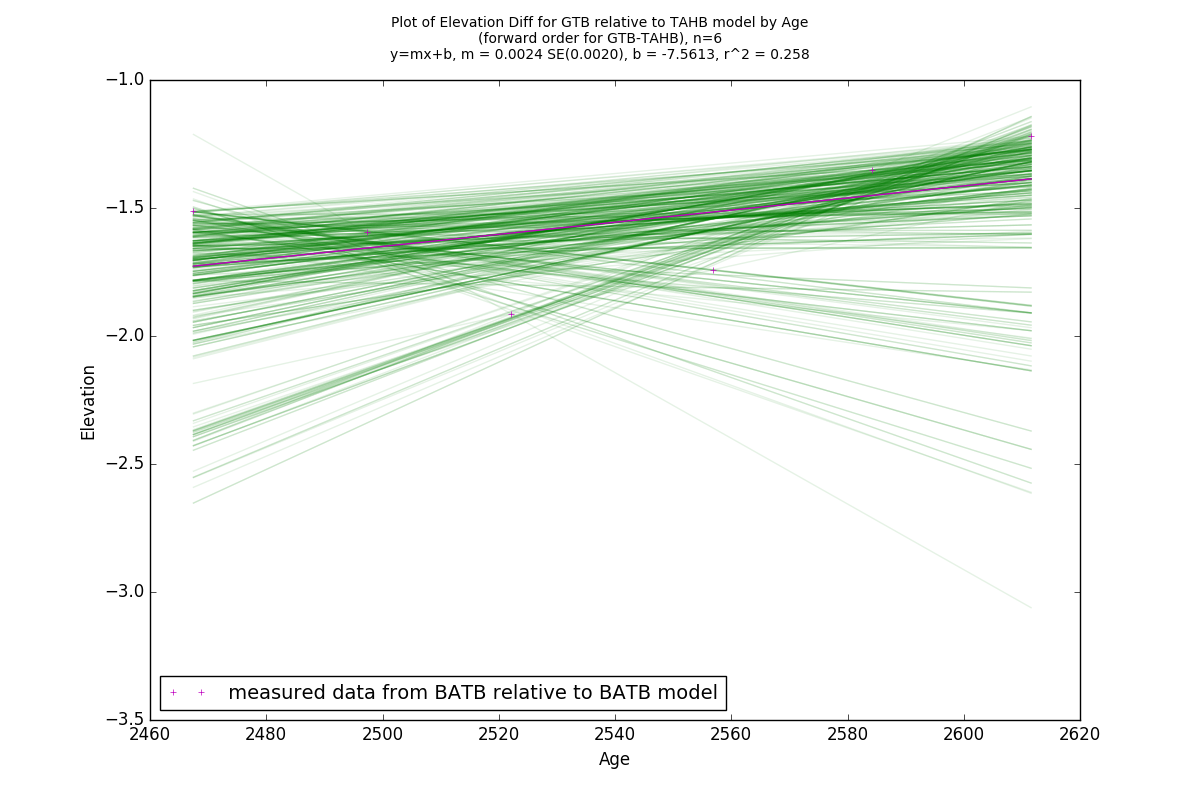
\includegraphics[width=0.9\linewidth]{data/gias/theGIA_GTB_relative_to_TAHB.png}
	\caption{Differences in elevation measured from the GTB data to the TAHB model}
	\label{fig:gias_GTBxTAHB}
\end{figure}
\newpage


\begin{figure}[h]
	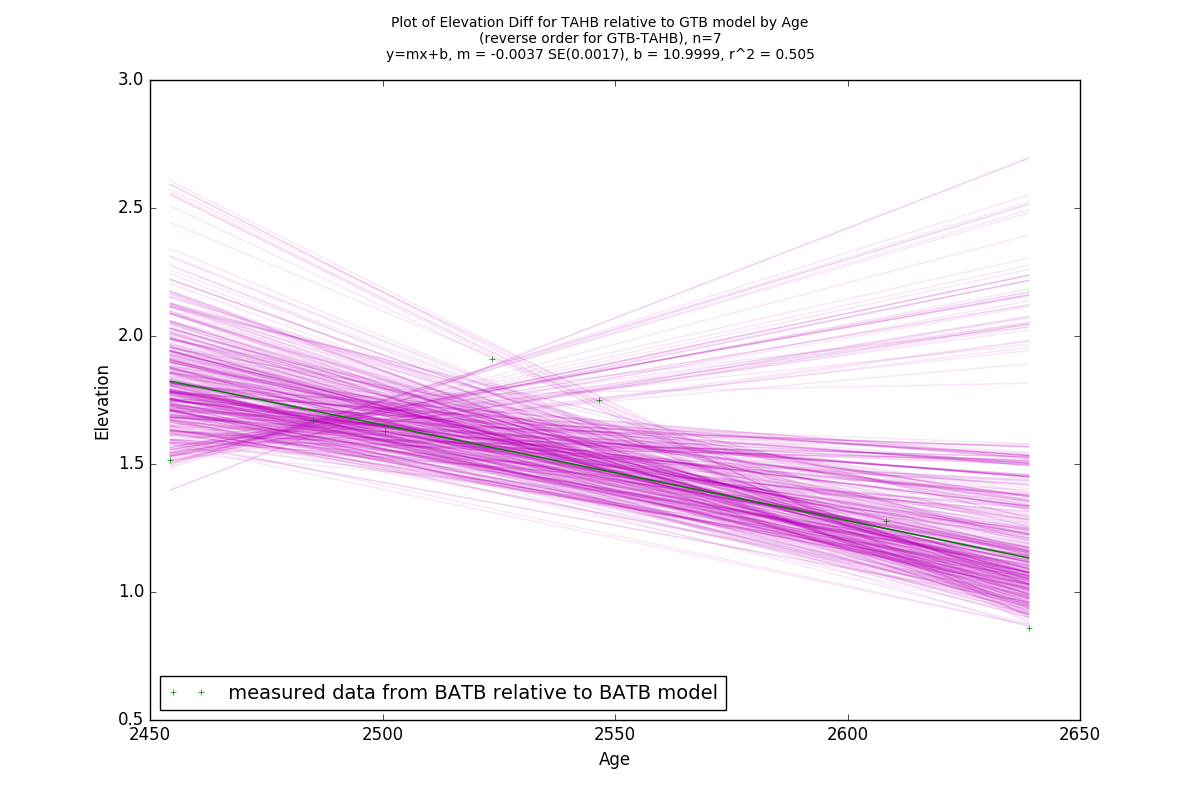
\includegraphics[width=0.9\linewidth]{data/gias/theGIA_TAHB_relative_to_GTB.png}
	\caption{Differences in elevation measured from the TAHB data to the GTB model}
	\label{fig:gias_TAHBxGTB}
\end{figure}
\newpage


\begin{figure}[h]
	\makebox[\textwidth]{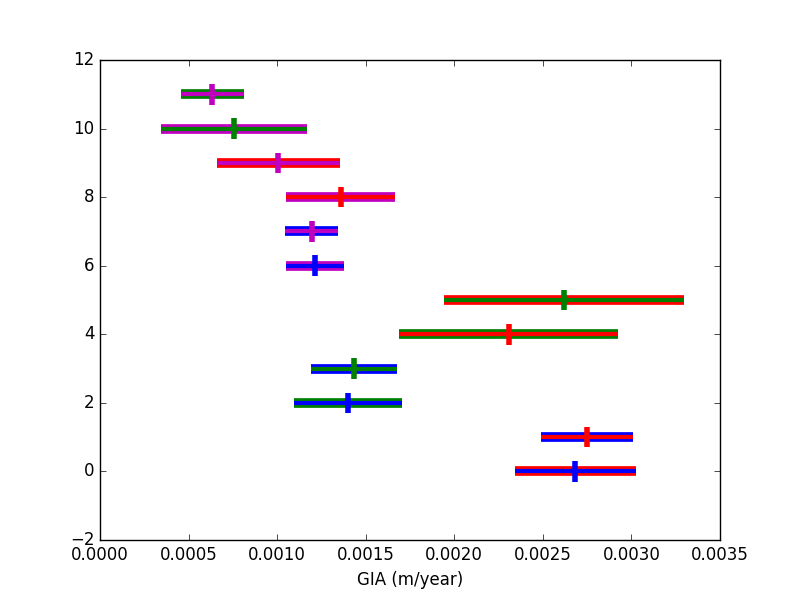
\includegraphics[width=0.6\paperwidth]{data/intervals.png}}
	\caption{95p Confidence intervals on GIA rates obtained from site comparisons}
	\label{fig:intervalsGIA}
\end{figure}


\newpage


\newpage

\subsubsection{Summary of calculated GIA values}

In Figure \ref{fig:myGIARates}, the values for relative GIA produced by this paper are
visualized by plotting the absolute value range of GIA rates between each site
as a line between sites on the map with the corresponding value next to it.

\begin{figure}[h]
	\makebox[\textwidth]{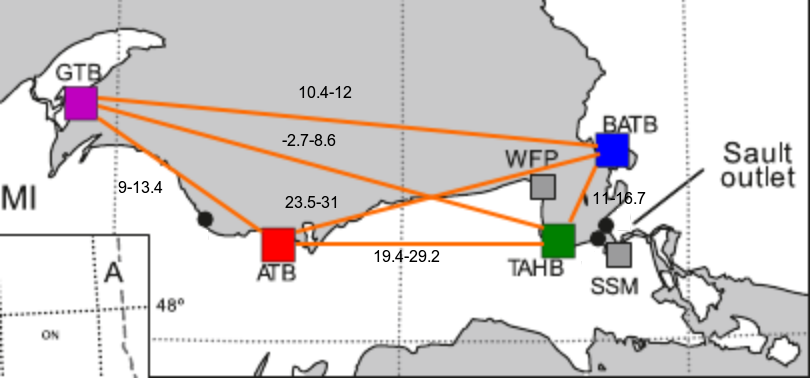
\includegraphics[width=0.72\paperwidth]{johnstonLaurentianMapWithMyGIARates.png}}
	\caption{Relative GIA Rates produced by this papers method, all values reported in cm/century}
	\label{fig:myGIARates}
\end{figure}
\newpage

The equivalent values for rates between sites as produced by Mainville \& Craymer
are inferred from subtracting the difference in contour between sites as shown in
Figure \ref{fig:craymerGIARatesBigPlot}, and are presented in Figure \ref{fig:craymerGIARates}.

\begin{figure}[h]
	\makebox[\textwidth]{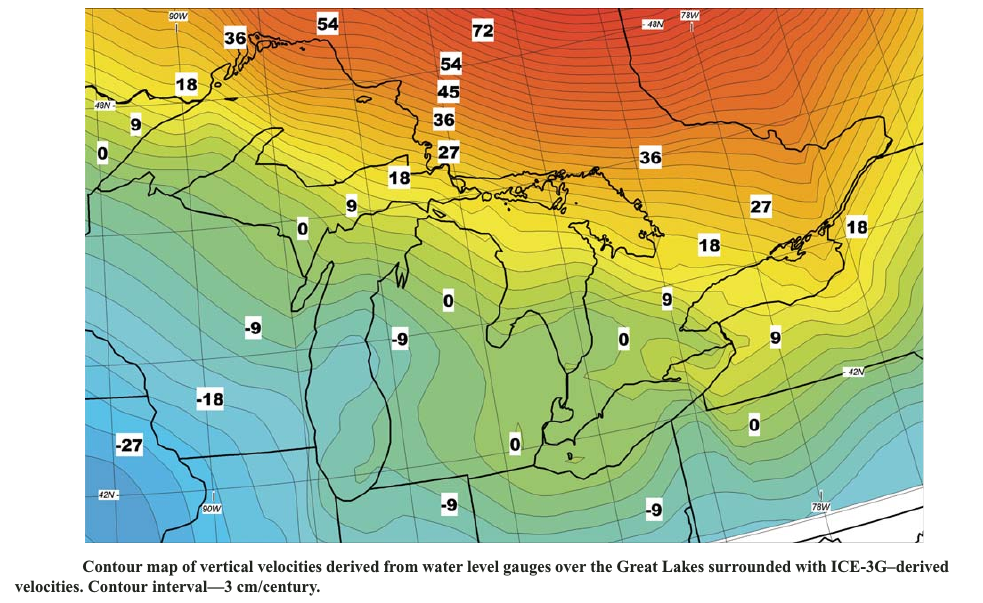
\includegraphics[width=0.72\paperwidth]{mainvilleGias.png}}
	\caption{Relative GIA Rates produced by Mainville \& Craymer, all values reported in cm/century (reproduced from Mainville \& Craymer, 2005)}
	\label{fig:craymerGIARatesBigPlot}
\end{figure}

\begin{figure}[h]
	\makebox[\textwidth]{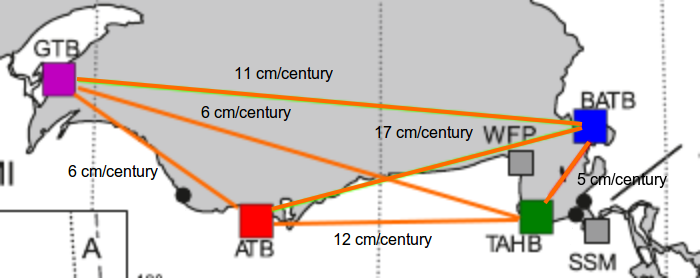
\includegraphics[width=0.72\paperwidth]{johnstonLaurentianMapWithCraymerGIARates.png}}
	\caption{Relative GIA Rates between this papers sites as reported by Mainville \& Craymer.}
	\label{fig:craymerGIARates}
\end{figure}
\newpage



Finally, the results of the analysis conducted in the previous section are summarized in
Figure \ref{fig:intervalsGIA}, which shows confidence intervals on absolute values of
rates of GIA for each and every site comparison calculated in Section 4. Each
pair of site comparisons is grouped in vertical order in order to show how each pair
of intervals overlaps, the range of GIA values in which they overlap is used as
the estimate of the absolute value GIA rate between the given pair of sites.

\newpage

\begin{figure}[H]
	\makebox[\textwidth]{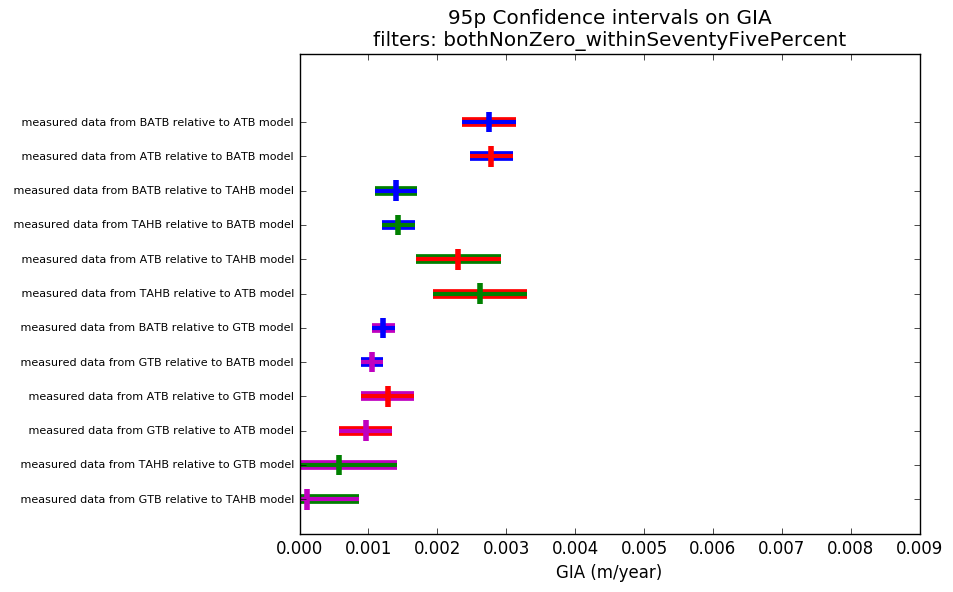
\includegraphics[width=0.6\paperwidth]{data/bothNonZero/withinSeventyFivePercent/gias/intervals.png}}
	\caption{Confidence intervals at the 95 \% confidence level for relative GIA rates obtained from 12 intra-site comparisons across 4 sites.}
	\label{fig:intervalsGIA}
\end{figure}

Comparing this papers results with those of Mainville \& Craymer, the value of
GIA reported by Mainville \& Craymer fell within the range reported by this paper
for 2 of the 6 pairs of sites (GTB \& TAHB and GTB \& BATB). For the remaining
four pairs of sites, the 95p confidence intervals on GIA calculated by this paper
tended to be larger than the equivalent values in Mainville \& Craymer, 
(namely ATB \& BATB, GTB \& ATB, and TAHB \& BATB) and sometimes much larger
(such as between ATB \& TAHB).

Given that the results of this paper are all on the same order of magnitude with
those reported by Mainville \& Craymer using data over a much shorter timescale,
this papers method can be inferred to be reasonably effective, but the
differences do need to be considered. These discrepancies may be an indication 
that the process of GIA in the LGL region behaved differently in the past than
in the more recent sample of time looked at by Mainville \& Craymer. One
particular area where significant
disagreement occurs is between sites ATB, BATB, and TAHB, especially in the much
larger values produced by this paper between ATB-BATB and ATB-TAHB. Given that both
of these site combinations are separated by an East-West line, this could imply
that the location of the center of the Laurentide Ice Sheet during the last glaciation being to the
north and west of Lake Superior had a stronger effect on the overall process of
rebound than the simple fact that areas to the north were more likely to be
depressed by the weight of ice sheets than areas further south. 

This interpretation should be taken with caution, given that the values produced
by this paper
may also be affected by differing quality of each intra-site measurement. Quality
of each GIA measurement is a subjective property, but it can be inferred that comparisons
that use as many data points as possible, which are evenly spread across as many 
200 year bins as possible, and have even quality between forward 
and reverse comparisons are more trustworthy than those that fail one or more of
those criteria. With that in mind, in the opinion of the Author of this paper,
the comparisons between GTB \& TAHB, GTB \& BATB, and TAHB \& ATB are of lesser
quality relative to the others. Coincidentally, two of these three comparisons
are those that agreed with Mainville \& Craymer, being lower in relative terms than
the rest of the comparisons. This could be interpreted to mean that the process of
GIA occurred at a higher rate over the longer periods of time studied by the
method of Johnston et al (2012) than it did over the shorter (and more recent)
span of time studied by that of Mainville \& Craymer (2005). Ultimately, this
conclusion is still an interpretation however, and the best method of determining
whether discrepancies between this papers method and previous ones would be to 
repeat the process with a dataset with better data coverage. One possible method
of accomplishing this would be further collection of data from sites already studied
in Johnston et al (2012), and by combining the data gathered from strandplains
closely spaced together around the lake basin.




\end{document}
